%%%%%%%%%%%%%%%%%%%%
%
% $Autor: Wings $
% $Datum: 2020-07-24 09:05:07Z $
% $Pfad: GDV/Vortraege/latex - Ausarbeitung/Kapitel/KreisStrategie.tex $
% $Version: 4732 $
%
%
%%%%%%%%%%%%%%%%%%%



\chapter{Verrundung mit einem Kreisbogen}

%todo Siehe \cite{Walton:2009} p.88, chapter 2.1.

\section{Gleichungen}

Die Verrundung mit einem Kreisbogen ist eine einfache Variante der Glättung von Ecken. Diese Variante ermöglicht die Bearbeitung und die Erzeugung von Dateien gemäß DIN 66025. Zur Glättung werden stets drei Punkte $P_0$ und $S$ und $P_1$ betrachtet, damit ergibt sich ein symmetrisches Hermite-Problem. Gemäß Satz \ref{StrategySymmetricDefStandardHP} wird vorausgesetzt, dass es sich in der Standardform $HP(L,\alpha)$ befindet.
 
 \bigskip
 
 
 
 \begin{figure}[h]
 %\centering
 %\includegraphics[width=.9\textwidth]{Sin2/Eckenglaettung11}
 
 
 \begin{center}
   \begin{tikzpicture}[scale=2]
 
     \coordinate[label=left:$P_0$]  (P0) at (2,0);
     \coordinate[label=right:$S$] 
        (PS) at (4,0);
     \coordinate[label=left:$P_1$] (P1) at (3.0,1.75);
     \coordinate[label=left:$M$] (M) at (2.0,1.2);
     
     \coordinate%[label=left:$P_i$]
       (P01) at
     ({4*(1.-0.5)+2.309265589*0.5*cos(-30)}, {2.309265589*0.5+2.309265589*0.5*sin(-30)});
     
     \coordinate[label=left:$\frac{\alpha}{2}$] (alpha) at (3.7,0.1);
 
     \coordinate[label=below:$L$](c) at ($ (P0)!.5!(PS) $);
     \coordinate[label=above:$r$] (b) at ($ (PS)!.75!(M) $);
     \coordinate[label=above:$+$] (b1) at ($ (PS)!.5!(M) $);
     \coordinate[label=above:$\varepsilon$] (b2) at ($ (PS)!.25!(M) $);
     \coordinate[label=left:$r$](a) at ($ (P0)!.5!(M) $);
 
     % draw the background
     \draw [line width=1.0pt] (P0) -- (PS);
     \draw [line width=1.0pt] (PS) --(P1);
     \draw [dotted,line width=1.0pt,blue] (PS) --(P01);
     \draw [line width=1.0pt,blue] (P01) --(M);
     \draw [line width=1.0pt,blue] (P0) --(M);
 %    \node[draw,circle through={(M)}] (Zentrum) {};
 
 
    \draw [red,line width=1.5pt,domain=-90:30] plot ({4*(1.-0.5)+2.309265589*0.5*cos(\x)}, {2.309265589*0.5+2.309265589*0.5*sin(\x)});
 
    \draw [green,line width=0.5pt,domain=180:150] plot ({4*(1.)+0.75*cos(\x)}, {0.75*sin(\x)});
 
     \node (P0) at (P0) {$\bullet$};
     \node (PS) at (PS) {$\bullet$};
     \node (M) at (M) {$\bullet$};
     \node (P1) at (P1) {$\bullet$};
 
   \end{tikzpicture}
 \end{center}
 \caption{Glättung einer Ecke mit Hilfe eines Kreisbogens - Dreieck}\label{KreisglaettungDreieck}
 \end{figure}
 
 
 Die Abbildung \ref{KreisglaettungDreieck} stellt die Situation dar.  Die Punkte $P_0$, $S$ und $P_1$ sind gegeben. Der eingeschlossene  Winkel $\alpha = \angle(P_0;S;P_1)$ sowie der Abstand $L=\|\|S-P_0\|\|  =\|\|P_1-S\|\|$ sind in der Grafik dargestellt.  Der rote Kreisbogen ist das gewünschte Ergebnis. Der Abstand seines Mittelpunkts $M$ zu $S$ beträgt dann $r+\varepsilon$, wobei $r$ der Radius des Kreisbogens und $\varepsilon$ die vorgegebene Toleranz ist. Somit erhalten wir ein rechtwinkliges  Dreieck $P_0SM$, dessen Kantenlängen $L$, $r+\varepsilon$ und $r$  sind.
 
 \bigskip
 
 Gemäß der Definition des Sinus und des Tangens folgt:
 
 $$\sin\left(\frac{\alpha}{2}\right)= \frac{L}{r+\varepsilon}
 \qquad \hbox{und}\qquad \tan\left(\frac{\alpha}{2}\right)= \frac{L}{r}$$
 
 $$\Leftrightarrow\quad 
 \varepsilon = \frac{L}{\sin\left(\frac{\alpha}{2}\right)} - r
 \qquad \hbox{und}\qquad 
  r = \cot\left(\frac{\alpha}{2}\right) L$$
 
 Die beiden Gleichung können zusammengefasst werden, so dass sich folgende Bedingungen  ergeben:
 
 $$\varepsilon = L \cdot \frac{1-\cos\left(\frac{\alpha}{2}\right)}{\sin\left(\frac{\alpha}{2}\right)}
 \qquad \hbox{bzw.} \qquad  L = \varepsilon \cdot \frac{\sin\left(\frac{\alpha}{2}\right)}{1-\cos\left(\frac{\alpha}{2}\right)}$$
 
 Damit ergibt sich für den Radius die Gleichung:
 
 $$r = L \cdot \cot\left(\frac{\alpha}{2}\right)
 = L \cdot \sqrt{\frac{1-\cos(\alpha)}{1+\cos(\alpha}}
 = L \cdot \frac{\sin(\alpha)}{1+\cos(\alpha)} = L \cdot \frac{P_{1,x}}{P_{1,y}}$$
 
 
 Der Faktor zum Umrechnung von $L$ und $\varepsilon$ kann mit Hilfe trigonometrischer Umformungen  vereinfacht werden.
 
 
 \bigskip
 
 
 $$\frac{1-\cos\left(\frac{\alpha}{2}\right)}{\sin\left(\frac{\alpha}{2}\right)}
 =
 \frac{1-\sqrt{\frac{1-\cos(\alpha)}{2}}}{\sqrt{\frac{1+\cos(\alpha)}{2}}}
 =
  \frac{\sqrt{2}-\sqrt{1-\cos(\alpha)}}{\sqrt{1+\cos(\alpha)}}
 = 
 \frac{\sqrt{1+\cos(\alpha)}-\sin(\alpha) }{1+\cos(\alpha)}
 $$
 
 Durch den Vergleich mit dem symmetrischen Hermite-Problem in Standardform ergibt sich dann die folgende Notation:
 
  
 $$\frac{1-\cos\left(\frac{\alpha}{2}\right)}{\sin\left(\frac{\alpha}{2}\right)}
 =
 \frac{\sqrt{P_{1,x}}-P_{1,y}}{P_{1,x}}
 $$
 
 Die vorherigen Überlegungen werden nun im nachfolgenden Satz zusammengefasst.
 
 \bigskip
 
 \SATZ{\label{KreisstrategieKreis}
   Es sei  ein symmetrisches Hermite-Problem $(P_0,\, \vec{t}_0,\,P_1,\, \vec{t}_1,S,L)$ gegeben. Ohne Einschränkung der Allgemeinheit liegt es in der Standardform

 $$\left\{\binom{0}{0},\, \binom{1}{0},\,
\binom{L+L\cdot \cos(\alpha)}{L\cdot \sin(\alpha)},\, \binom{\cos(\alpha)}{\sin(\alpha)},\, \binom{L}{0},L\right\}$$

mit $L\in \R^{>0}$ und $\alpha \in (-\pi;\, \pi] $ vor.
  
  \medskip
  
  
  Dann kann ein Kreisbogen gefunden werden, der die Punkte $P_0$ und $P_1$  verbindet, die gleichen Tangentenrichtungen in den beiden  Punkten besitzt.
  
  \medskip
  
  Für die Kreisbogen gilt:
  
  $$r= L \cdot \left| \frac{P_{1,x}}{P_{1,y}}\right|; \quad 
    \phi_0 = -\sign(\alpha)  \cdot \frac{\pi}{2}; \quad
    \phi_1-\phi_0 
        = \sign(\alpha)  \cdot \pi - \alpha = \beta; $$
        
        $$
         M 
           = P_0 + \sign(\alpha) \cdot 
          r \cdot 
          \vec{t}_0^\perp 
          = \sign(\alpha) \cdot 
                    r \cdot \binom{0}{1}
          $$
 }
 
 
 \bigskip
 
 
 Aus der Vorgabe des Abstand $L$ kann, wie in Satz \ref{KreisstrategieKreis} dargestellt, der maximale Fehler berechnet werden. Gemäß der Herleitung ist es auch möglich, den maximalen Fehler $\varepsilon$ vorzugeben und daraus den maximalen Abstand $L$ zu  bestimmen.
 
 
 \bigskip
 
  \SATZ{\label{KreisstrategieLEps} Es sei  ein symmetrisches Hermite-Problem $(P_0,\, \vec{t}_0,\,P_1,\, \vec{t}_1,S,L)$  gegeben. Ohne Einschränkung der Allgemeinheit liegt es in der Standardform
  
   $$\left\{\binom{0}{0},\, \binom{1}{0},\,
  \binom{L+L\cdot \cos(\alpha)}{L\cdot \sin(\alpha)},\, \binom{\cos(\alpha)}{\sin(\alpha)},\, \binom{L}{0},L\right\}$$
  
  mit $L\in \R^{>0}$ und $\alpha \in (-\pi;\, \pi] $ vor.
   
   \medskip
   
   \begin{itemize}
     \item [a)] Es sei der maximale Fehler $\varepsilon$ vorgegeben. Der maximale Abstand $L$, für den ein Kreisbogen gemäß Satz \ref{KreisstrategieKreis} existiert, der den Fehler berücksichtigt, ist gegeben durch:
         
         $$L(\varepsilon,\alpha) 
           =
           \varepsilon \cdot \frac{P_{1,x}}{\sqrt{P_{1,x}}-P_{1,y}}
           =
           \varepsilon \cdot \frac{L+L\cdot \cos(\alpha)}{\sqrt{L+L\cdot \cos(\alpha)}-L+L\cdot \cos(\alpha)}
         $$
          
      \item [b)] Bei der Vorgabe des Abstands $L$ ergibt sich der folgende,  maximale    Fehler:         
         
          $$
            \varepsilon(L,\alpha) 
            = 
            L \cdot  \frac{\sqrt{P_{1,x}}-P_{1,y}}{P_{1,x}}
            =
            L \cdot \frac{\sqrt{L+L\cdot \cos(\alpha)}-L+L\cdot \cos(\alpha)}{L+L\cdot \cos(\alpha)}
           $$

          
         
     
   \end{itemize}
} 
 
 
%\section{Kreis}
%\subsection{Darstellung eines Punktes auf einem Kreis}
%Darstellung eines beliebigen Punktes auf einer Kurve in Abhängigkeit eines Parameters $\lambda$. \linebreak
%
%\begin{equation}
%\vec{p}(\lambda)=\binom{p_x(\lambda)}{p_y(\lambda)}
%\end{equation}
%
%
%Befindet sich der Punkt auf einem Kreis mit dem Radius r und dem Mittelpunkt $\vec{m}=\binom{m_x}{m_y}$ des Kreises auch der Ursprung des Koordinatensystem, so kann man jeden beliebigen Punkt auf dem Kreis in Abhängigkeit des Winkles $\alpha \in [0;2\pi]$  darstellen.\linebreak
%Die Funktion C($\alpha$) entspricht dann:
%
%\begin{equation}
%C(\alpha)=\vec{m}+r*\binom{p_x(\alpha)}{p_y(\alpha)}
%\end{equation}
%
%
%Der Punkt lässt sich in X und Y-Komponenten aufteilen
%
%\subsection{Implizite Kreisdarstellung}
%Mit Hilfe von Phytagoras ergibt sich die implizite Kreisdarstellung :
%
%\begin{equation}
%(p_x-m_x)^2+(p_y-m_y)^2=r^2
%\end{equation}
%
%Daraus ergibt sich für die Strecke vom Ursprung zu $p_x$ bzw. $p_y$:
%
%\begin{eqnarray}
%p_x=&m_x+r\cdot\cos(\alpha)\\
%p_y=&m_y+r\cdot\sin(\alpha)
%\end{eqnarray}
%
%
%
%
%\subsection{Explizite Kreisdarstellung}
%Eine Funktion für die für die explizite Darstellung eines Punktes auf einem Kreis lautet dann:
%
%\begin{equation}
%C(\alpha)=\vec{m}+r\cdot\binom{\cos(\alpha)}{\sin(\alpha)}
%\end{equation}
%Siehe hierzu auch Kapitel 5. Kreis 
%
%%\subsection{Kreisbogen}
%
%\begin{equation}
%B: \begin{cases}
%[\varphi_0; \varphi_0 + \alpha] &\rightarrow \mathbb{R}^2 \\
%\varphi&\mapsto\vec{m}+r\cdot\binom{\cos(\varphi)}{\sin(\varphi)}
%\end{cases}
%\end{equation}




%todo Quelle

\bigskip

Aus diesen Überlegungen ergeben sich Einschränkungen für den Einsatz dieser Strategie, die in der folgenden Bemerkung zusammengefasst sind.


\bigskip



\Bemerkung
{
  Folgende Bedingungen zum Anwenden der Strategie eines Kreises müssen erfüllt sein:

  \begin{itemize}
    \item [a)] $$P_0 \neq P_1$$
    \item [b)] $$ \vec{t}_0 = -\vec{t}_1\quad \Leftrightarrow \quad \alpha = 0$$
    \item [c)] $$ \vec{t}_0 =  \vec{t}_1\quad \Leftrightarrow \quad \alpha = \pi$$
  \end{itemize}
}


\section{Bewertung}

Die Verrundung mittels eines Kreisbogens führt zu einem stetigen Verlauf der Winkeländerung. Die Abbildung \ref{KreisstrategieWinkel} stellt dies dar.

\bigskip

\begin{figure}
  \begin{center}
    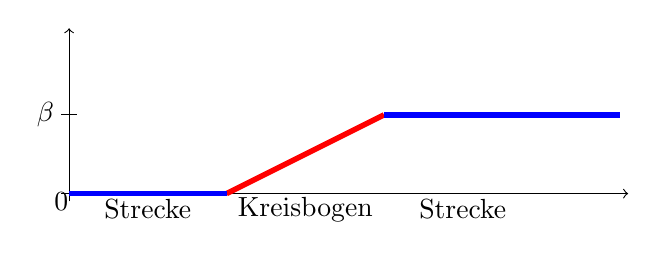
\begin{tikzpicture}
       \draw [->] (0,-0.1) -- (0,2.1);
       \draw [->] (-0.1,0) -- (7.1,0);
       \draw (-0.1,1) -- (0.1,1);
       
       \node (R) at (-0.3,1) {$\beta$};
       \node (O) at(-0.1,-0.1) {$0$};
       
       
       \node (P0) at (1,-0.2) {Strecke};
       \node (P0) at (3,-0.2) {Kreisbogen};
       \node (P0) at (5,-0.2) {Strecke};
       \draw [line width=2pt,color=red] (2,0) -- (4,1);
       \draw [line width=2pt,color=blue] (0,0) -- (2,0);
       \draw [line width=2pt,color=blue] (4,1) -- (7,1);
       
    \end{tikzpicture}
  \end{center}
  \caption{Winkeländerung bei einer  Verrundung mit einem Kreisbogen }\label{KreisstrategieWinkel}
\end{figure}

\bigskip

Durch die Verrundung mit einem Kreisbogen wird ist der Krümmungsverlauf der Kurve nicht stetig. Die Abbildung \ref{KreisstrategieKruemmung} zeigt, dass die Krümmung im Bereich der Strecken $0$ ist und auf dem Kreisbogen konstant mit dem Wert $\frac{1}{r}$, wobei $r$ der Radius des eingesetzten Kreisbogens ist. Aufgrund der Formel $a=\frac{v^2}{r}$ für eine Bewegung auf einem Kreisbogen weist der Beschleunigungsverlauf bei einer konstanten Bahngeschwindigkeit Stetigkeitssprüngen an  den Übergängen aus.


\begin{figure}
  \begin{center}
    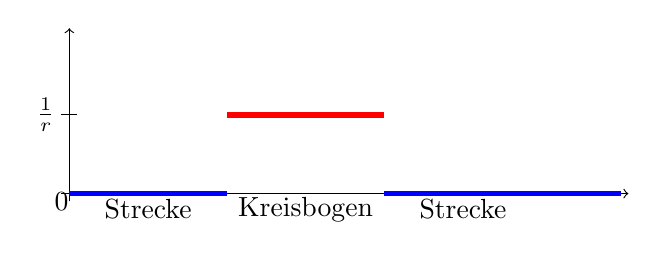
\begin{tikzpicture}
       \draw [->] (0,-0.1) -- (0,2.1);
       \draw [->] (-0.1,0) -- (7.1,0);
       \draw (-0.1,1) -- (0.1,1);
       
       \node (R) at (-0.3,1) {$\frac{1}{r}$};
       \node (O) at(-0.1,-0.1) {$0$};
       
       
       \node (P0) at (1,-0.2) {Strecke};
       \node (P0) at (3,-0.2) {Kreisbogen};
       \node (P0) at (5,-0.2) {Strecke};
       \draw [line width=2pt,color=red] (2,1) -- (4,1);
       \draw [line width=2pt,color=blue] (0,0) -- (2,0);
       \draw [line width=2pt,color=blue] (4,0) -- (7,0);
       
    \end{tikzpicture}
  \end{center}
  \caption{Krümmungsverlauf bei der Verrundung mit einem Kreisbogen}\label{KreisstrategieKruemmung}
\end{figure}



\bigskip




In Abhängigkeit der Winkeländerung $\beta$ an der Ecke $S$ und der Toleranz $\varepsilon$ kann die maximale Länge der Verkürzung der Strecken berechnet werden. Die Abbildung~\ref{KreisstrategieL} zeigt das zugehörige Diagramm, wobei die Toleranz $\varepsilon$ auf den Wert $1$ gesetzt ist.
 
 
\begin{figure}
  \begin{center}
    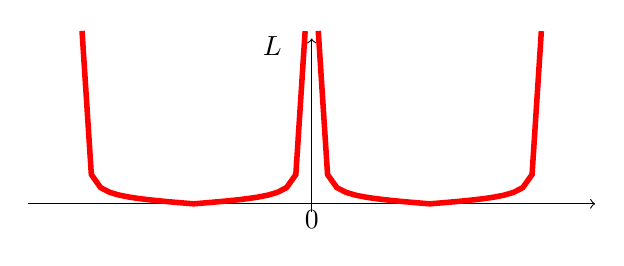
\begin{tikzpicture}[declare function ={Leps(\a) =sqrt(abs(sin(180-\a)*(sin(180-\a)-1)))/abs(10*sin(180-\a)-1);}]
    \draw [->] (3.5,-0.1) -- (3.5,2.1);
    \draw [->] (-0.1,0) -- (7.1,0);
    
    \node (R) at (3.0,2) {$L$};
    \node (O) at(3.5,-0.2) {$0$};
    
    \draw [red,line width=2pt,domain=175:5] plot({3.5-\x/60},{Leps(\x)});
    \draw [red,line width=2pt,domain=5:175] plot({3.5+\x/60},{Leps(\x)});
  
    
    
    \end{tikzpicture}
  \end{center}
  \caption{Maximaler Bereich für die Verrundung mit einem Kreisbogen - $L(\varepsilon=const, \alpha)$}\label{KreisstrategieL}
\end{figure}


\bigskip

Der Bereich, der zur Verfügung gestellt wird, kann auch vorgegeben werden. In Abhängigkeit des Abstands $L$ vom Eckpunkt $S$ kann die Abweichung $\varepsilon$ berechnet werden. Die Abbildung \ref{KreisstrategieEps} stellt die Funktion in Abhängigkeit von $L$ und des Winkels $\alpha$ dar.



 
\begin{figure}
  \begin{center}
    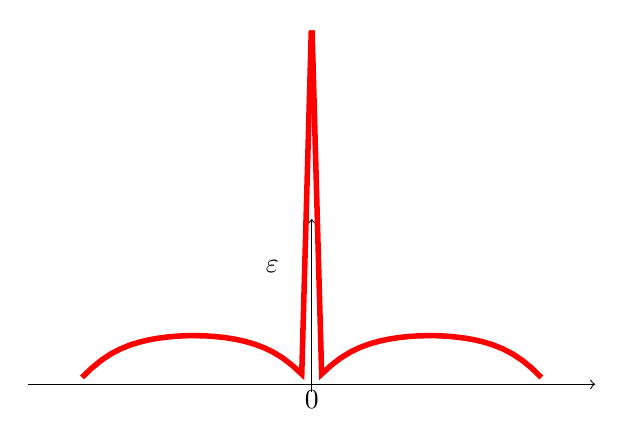
\begin{tikzpicture}[declare function ={EpsL(\x) =sqrt(1+1/(4*sin(180-\x)*sin(180-\x)))-1/(2*sin(180-\x));
    }]
    \draw [->] (3.5,-0.1) -- (3.5,2.1);
    \draw [->] (-0.1,0) -- (7.1,0);
    
    \node (R) at (3,1.5) {$\varepsilon$};
    \node (O) at(3.5,-0.2) {$0$};
    
   \draw [red,line width=2pt,domain=0.3:175] plot({3.5-\x/60},{EpsL(\x)/1});
   \draw [red,line width=2pt,domain=0.3:175] plot({3.5+\x/60},{EpsL(\x)/1});
    
    
    
    \end{tikzpicture}
  \end{center}
  \caption{Abweichung bei Vorgabe des Abstands $L$ bei der Verrundung mit einem Kreisbogen}\label{KreisstrategieEps}
\end{figure}


Die Abbildungen \ref{KreisstrategieL} und \ref{KreisstrategieEps} zeigen die Kurven der Länge in Abhängigkeit der Winkeländerung bei einer festen Toleranz und den Fehler in Abhängigkeit der Winkeländerung bei vorgegebenen Länge. Falls die Winkeländerung minimal ist, dann  ist der Fehler oder die Länge $L$ extrem. In diesem Fall ist eine Verrundung mittels eines Kreisbogens nicht möglich. Um eine sinnvolle Strategie zu entwickeln, muss eine minimale Winkeländerung vorgegeben werden, ab der eine Verrundung mit einem Kreisbogen erlaubt ist. Ebenso ist eine maximale
Winkeländerung zu definieren. Denn bei einer Winkeländerung von $\pm \pi$ handelt sich um eine Kehre. in diesem Fall ist eine Verrundung auch nicht 
möglich.




\section{Beispiele}

\BEISPIEL
{
Es sei das symmetrische Hermite-Problem 

   $$\left\{\binom{0}{0},\, \binom{1}{0},\,
\binom{6.0+6.0\cdot \cos\left(\frac{2}{3}\pi\right)}{6.0\cdot \sin\left(\frac{2}{3}\pi\right)},\, \binom{\cos\left(\frac{2}{3}\pi\right)}{\sin\left(\frac{2}{3}\pi\right)},\, \binom{6.0}{0},6.0\right\}$$

mit $L=6$ und $\alpha=\frac{2}{3}\pi$ gegeben.

Für den Verrundungskreisbogen folgt:

$$M=\binom{0}{3,4641}; \quad r=3,46412;\quad \phi_0 = -\frac{\pi}{2}; \quad \alpha=\frac{2}{3}\pi$$


\begin{center}
  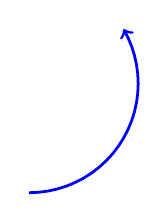
\begin{tikzpicture}[scale=0.4]
    \begin{scope}
      \HermiteSym{1}{120}
    \end{scope}

    \begin{scope}[shift={(12cm,0cm)}]
      \HermiteSym{1}{120}
      \draw [blue,line width=1pt,domain=-90:30,->] plot ({0+3.464101612*cos(\x)}, {3.464101612+3.464101612*sin(\x)});
    \end{scope}
  \end{tikzpicture}
\end{center}
}


\BEISPIEL
{
  Es sei das symmetrische Hermite-Problem 
  
  $$\left\{\binom{0}{0},\, \binom{1}{0},\,
  \binom{6.0+6.0\cdot \cos\left(\frac{7}{18}\pi\right)}{6.0\cdot \sin\left(\frac{7}{18}\pi\right)},\, \binom{\cos\left(\frac{7}{18}\pi\right)}{\sin\left(\frac{7}{18}\pi\right)},\, \binom{6.0}{0},6.0\right\}$$
  
  mit $L=6$ und $\alpha=\frac{7}{18}\pi$ gegeben.
  
  Für den Verrundungskreisbogen folgt:
  
  $$M=\binom{0}{8,5689}; \quad r=8,5689;\quad \phi_0 = -\frac{\pi}{2}; \quad \alpha=\frac{7}{18}\pi$$
  
  
  \begin{center}
    \begin{tikzpicture}[scale=0.4]
    \begin{scope}
    \HermiteSym{1}{70}
    \end{scope}
    
    \begin{scope}[shift={(12cm,0cm)}]
    \HermiteSym{1}{70}
    \draw [blue,line width=1pt,domain=-90:-20,->] plot ({0+8.568888035*cos(\x)}, {8.568888035+8.568888035*sin(\x)});
    \end{scope}
    \end{tikzpicture}
  \end{center}
}



\BEISPIEL
{
  Es sei das symmetrische Hermite-Problem 
  
  $$\left\{\binom{0}{0},\, \binom{1}{0},\,
  \binom{6.0+6.0\cdot \cos\left(\frac{1}{9}\pi\right)}{6.0\cdot \sin\left(\frac{1}{9}\pi\right)},\, \binom{\cos\left(\frac{1}{9}\pi\right)}{\sin\left(\frac{1}{9}\pi\right)},\, \binom{6.0}{0},6.0\right\}$$
  
  mit $L=6$ und $\alpha=\frac{1}{9}\pi$ gegeben.
  
  Für den Verrundungskreisbogen folgt:
  
  $$M=\binom{0}{34,0277}; \quad r=34,0277;\quad \phi_0 = -\frac{\pi}{2}; \quad \alpha=\frac{1}{9}\pi$$
  
  
  \begin{center}
    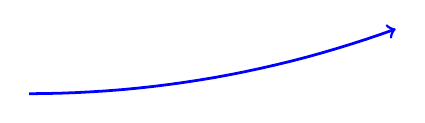
\begin{tikzpicture}[scale=0.4]
    \begin{scope}
    \HermiteSym{1}{20}
    \end{scope}
    
    \begin{scope}[shift={(12cm,0cm)}]
    \HermiteSym{1}{20}
    \draw [blue,line width=1pt,domain=-90:-70,->] plot ({0+34.02769092*cos(\x)}, {34.02769092+34.02769092*sin(\x)});
    \end{scope}
    \end{tikzpicture}
  \end{center}
}


\BEISPIEL
{
  Es sei das symmetrische Hermite-Problem 
  
  $$\left\{\binom{0}{0},\, \binom{1}{0},\,
  \binom{12.0}{0},\, \binom{1}{0},\, \binom{6.0}{0},6.0\right\}$$
  
  mit $L=6$ und $\alpha=0$ gegeben.
  
 Hier existiert kein Verrundungskreisbogen.
  
  
  \begin{center}
    \begin{tikzpicture}[scale=0.4]
    \begin{scope}
    \HermiteSym{1}{0}
    \end{scope}
    
    \end{tikzpicture}
  \end{center}
}



\BEISPIEL
{
  Es sei das symmetrische Hermite-Problem 
  
  $$\left\{\binom{0}{0},\, \binom{1}{0},\,
  \binom{6.0+6.0\cdot \cos\left(-\frac{1}{9}\pi\right)}{6.0\cdot \sin\left(-\frac{1}{9}\pi\right)},\, \binom{\cos\left(-\frac{1}{9}\pi\right)}{\sin\left(-\frac{1}{9}\pi\right)},\, \binom{6.0}{0},6.0\right\}$$
  
  mit $L=6$ und $\alpha=-\frac{1}{9}\pi$ gegeben.
  
  Für den Verrundungskreisbogen folgt:
  
  $$M=\binom{0}{-34,0277}; \quad r=34,0277;\quad \phi_0 = \frac{\pi}{2}; \quad \alpha=\frac{1}{9}\pi$$
  
  
  \begin{center}
    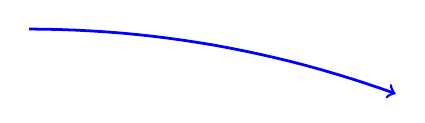
\begin{tikzpicture}[scale=0.4]
    \begin{scope}
    \HermiteSymNeg{1}{-20}
    \end{scope}
    
    \begin{scope}[shift={(12cm,0cm)}]
    \HermiteSymNeg{1}{-20}
    \draw [blue,line width=1pt,domain=90:70,->] plot ({0+34.02769092*cos(\x)}, {-34.02769092+34.02769092*sin(\x)});
    \end{scope}
    \end{tikzpicture}
  \end{center}
}



\BEISPIEL
{
  Es sei das symmetrische Hermite-Problem 
  
  $$\left\{\binom{0}{0},\, \binom{1}{0},\,
  \binom{6.0+6.0\cdot \cos\left(-\frac{7}{18}\pi\right)}{6.0\cdot \sin\left(-\frac{7}{18}\pi\right)},\, \binom{\cos\left(-\frac{7}{18}\pi\right)}{\sin\left(-\frac{7}{18}\pi\right)},\, \binom{6.0}{0},6.0\right\}$$
  
  mit $L=6$ und $\alpha=-\frac{7}{18}\pi$ gegeben.
  
  Für den Verrundungskreisbogen folgt:
  
  $$M=\binom{0}{-8,5689}; \quad r=8,5689;\quad \phi_0 = \frac{\pi}{2}; \quad \alpha=-\frac{7}{18}\pi$$
  
  
  \begin{center}
    \begin{tikzpicture}[scale=0.4]
    \begin{scope}
    \HermiteSymNeg{1}{-70}
    \end{scope}
    
    \begin{scope}[shift={(12cm,0cm)}]
    \HermiteSymNeg{1}{-70}
    \draw [blue,line width=1pt,domain=90:20,->] plot ({0+8.568888035*cos(\x)}, {-8.568888035+8.568888035*sin(\x)});
    \end{scope}
    \end{tikzpicture}
  \end{center}
}


\BEISPIEL
{
  Es sei das symmetrische Hermite-Problem 
  
  $$\left\{\binom{0}{0},\, \binom{1}{0},\,
  \binom{6.0+6.0\cdot \cos\left(-\frac{2}{3}\pi\right)}{6.0\cdot \sin\left(-\frac{2}{3}\pi\right)},\, \binom{\cos\left(-\frac{2}{3}\pi\right)}{\sin\left(-\frac{2}{3}\pi\right)},\, \binom{6.0}{0},6.0\right\}$$
  
  mit $L=6$ und $\alpha=-\frac{2}{3}\pi$ gegeben.
  
  Für den Verrundungskreisbogen folgt:
  
  $$M=\binom{0}{-3,4641}; \quad r=3,46412;\quad \phi_0 = \frac{\pi}{2}; \quad \alpha=-\frac{2}{3}\pi$$
  
  
  \begin{center}
    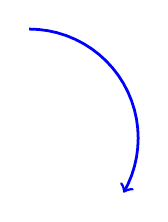
\begin{tikzpicture}[scale=0.4]
    \begin{scope}
    \HermiteSymNeg{1}{-120}
    \end{scope}
    
    \begin{scope}[shift={(12cm,0cm)}]
    \HermiteSymNeg{1}{-120}
    \draw [blue,line width=1pt,domain=90:-30,->] plot ({0+3.464101612*cos(\x)}, {-3.464101612+3.464101612*sin(\x)});
    \end{scope}
    \end{tikzpicture}
  \end{center}  
}



%todo Weiterführende Themen
%\section{Todo}
%\textcolor{red}{Kreis-Kreis-Übergang}
%\textcolor{red}{Gerade-Kreis-Übergang}
